\section{Methodology} \label{sec3}

In the previous section some issues were identified with the dataset. The \textit{Algorithms and Techniques} subsection details the algorithms that were used to remedy these issues. In this section we show the results that were acquired during data preprocessing.

The other important contribution of this section is the feature engineering part. This provides details about how the features from the dataset were extracted.

\subsection{Preprocessing the Portfolio Dataset} \label{sec3.1}

We do not use much data about the portfolio dataset. We do realize that some interesting features could have also been extracted from this data, however we decided to focus on other features of the data. In the full created feature vectors the offer that was received is one-hot-encoded to be able to feed it to the neural network. Also the duration of the offers is converted to hours to be able to use it with the transcript dataset where the timestamp is provided in hours instead of days.

\subsection{Preprocessing the Profile Dataset} \label{sec3.2}

Due to the reasons detailed in the previous section we removed the people who have spent more than a total of 300\$ or did not spend anything. With this we have removed 6.8\% of the profile and and 7.3\% of the transcript data. These are not very large percentages, so there are plenty of data remaining after this selection.

After this, we have one-hot-encoded the gender into the following categories: "F", "M", "O" and "U". 

Before filling up the "None" type values in the dataset, the age and income fields are standardized using sklearn's StandardScaler algorithm. The features before and after standardization can be seen on Figure \ref{fig9}

\begin{figure}[h]
	\centering
	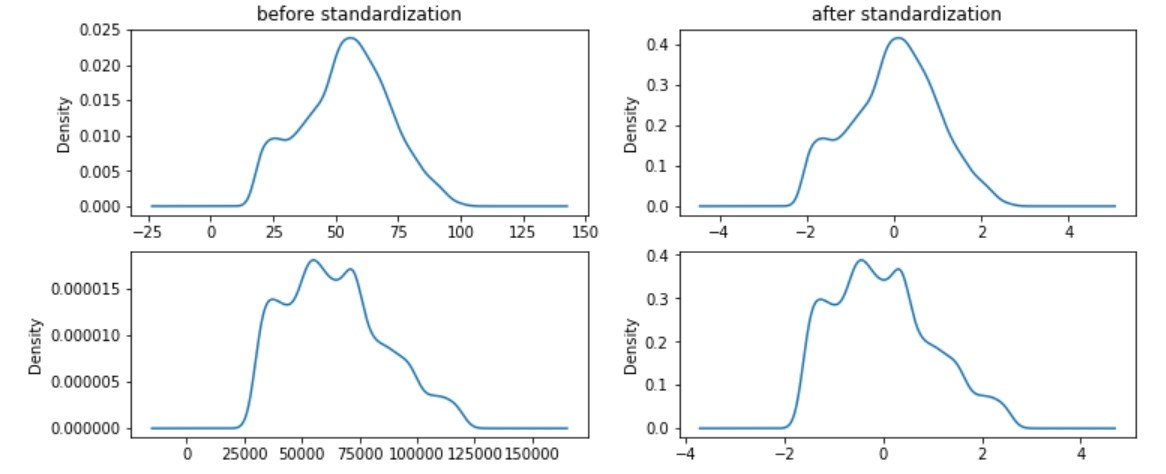
\includegraphics[width=0.8\textwidth]{fig/age_before_after.jpg}
	\vspace*{-0.1in}
	\caption{Age and income before and after standardization}
	\label{fig9}
	\vspace*{-0.2in}
	\bigskip
\end{figure}

After standardizing the age and income data, the missing values can be filled with the respective means. 

Next the membership length is calculated and since it was shown that it has a quite distorted distribution, it will be transformed using sklenarn's QuintileTransform algorithm. After that the resultant data is also standardized. The data before and after the transformation can be examined in Figure \ref{fig10}.

\begin{figure}[h]
	\centering
	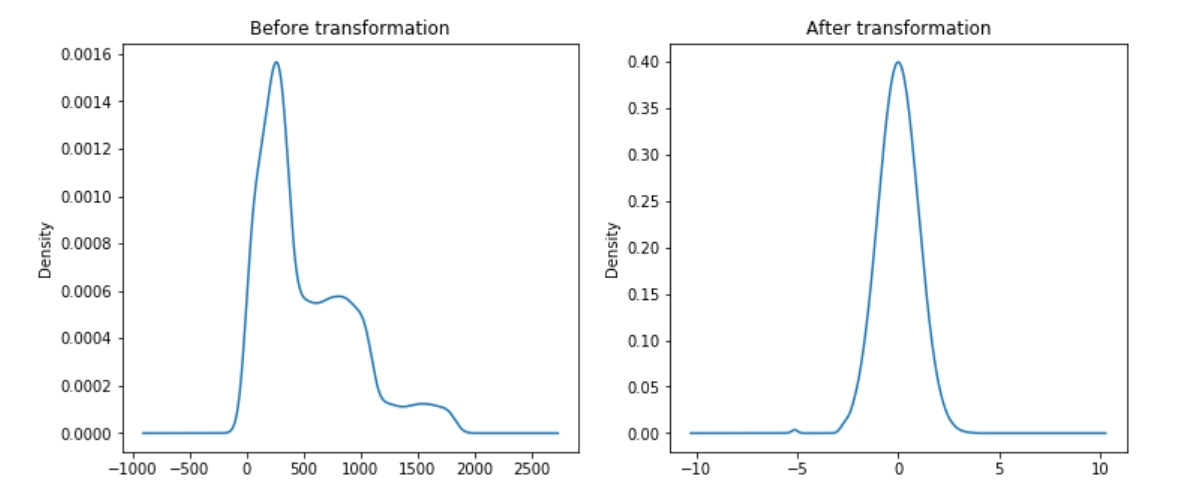
\includegraphics[width=0.8\textwidth]{fig/membership_before_after.jpg}
	\vspace*{-0.1in}
	\caption{Membership length before and after the transformation and standardization.}
	\label{fig10}
	\vspace*{-0.2in}
	\bigskip
\end{figure}

After the data was preprocessed and cleaned it is ready for handcrafted feature creation.

\subsection{Feature Engineering} \label{sec3.3}

A crutial part of out solution is the way the features and the corresponding labels are handcrafted from the raw data. In this subsection we define how the feature vector is composed and briefly introduce the algorithm that manufactures it from the raw dataset.

Our main goal is to be able to predict that if an offer would be sent to a specified costumer, what the costumers most probable reaction for receiving the offer would be. We are trying to classify each received offer into the 4 groups that were introduced int section \ref{sec1.2}. For this in a real life scenario we can not use data from the "future", but one has to make its prediction based on past experiences with the costumer. It is also possible that the costumer is fresh, that is the company does not yet have a record about this person yet, however we would also like to make predictions about that person. 

To achieve this, features are required which we assume that represent the costumers in detail and also are usable for costumers with different recorded history. To achieve this goal, we have chosen to create the features with the following procedure: 

First we pruned the datapoints from the transcript data where the offer was received so late, that its expiration date is out of the scope of the 30 day period. These offers are not representative in our point of view. Then we create a training point for every received offer, since every single received offer can be examined, how the costumer reacted to it. Hence, for every received offer we check, into which category it falls in the categories of section \ref{sec1.2}. After that we take the history (if there is any) of the person who received the offer only until that point when the offer was received. Than we create some representative features based on this history segment. The features that we create are as follows:

\begin{itemize}
	\item Personal data: Age, income, gender, membership length. These are the data that we have about every costumer irregardless of their recorded history length. (For new costumers these are the only relevant features that we have.)
	\item General costumer history: Some statistical data about the costumer's activity until the point the offer was received. It includes the following features:
		\subitem average amount spent
		\subitem number of offers received
		\subitem fraction of viewed and received offers
		\subitem fraction of completed and viewed offers
		\subitem fraction of completed but not viewed offers
	\item Costumer history in connection with this product. Some measuring numbers about the costumer's history with this received product. It includes the following features:
		\subitem number of offers received from this type
		\subitem fraction of viewed and received offers of this type
		\subitem fraction of completed and viewed offers of this type
		\subitem fraction of completed but not viewed offers of this type
	\item type of the offer in one-hot-encoding
\end{itemize}.

These features allow to represent a costumer quite in detail. With this method we have created 61324 training points for the model. The number of training points for the different classes can be seen in Figure \ref{fig11}

\begin{figure}[h]
	\centering
	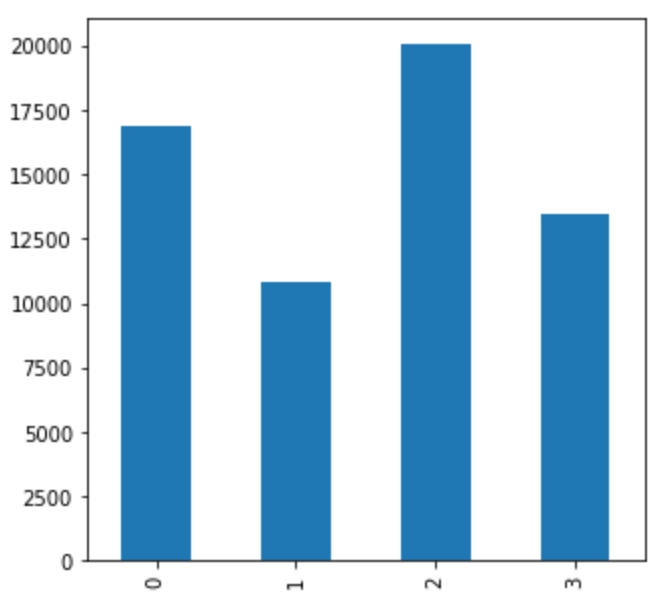
\includegraphics[width=0.5\textwidth]{fig/num_labels.jpg}
	\vspace*{-0.1in}
	\caption{Number of labels in the 4 classes.}
	\label{fig11}
	\vspace*{-0.2in}
	\bigskip
\end{figure}

The differences in the number of labels is going to be compensated during training.

We have also checked the correlation matrix of the generated features. We have found that the features are not much correlated, they are going to be sufficiently independent for training.

\subsection{Implementation} \label{sec3.4}
In this section we are going to provide some details how te project was implemented. Most of the implementation details are spread in this document, because we have found that the report is better readable in this way. Here however we provide some details on the technical workflow of implementation.

During implementation we have been working along the following workflow:
\begin{itemize}
	\item Data Exploration
	\item Feature Engineering
	\item Preparing the data for training
	\item splitting the data into training (80\%), validation (10\%) and test sets (10\%)
	\item Neural network implementation
	\item Iterating between hyperparameter tuning, relevant feature selection and training until we have found the best setup based on validation accuracy
	\item Testing the accuracy on the test set
	\item comparing the performance if the trained and the benchmark models.
\end{itemize}

We have mostly used python notebooks during implementation. The Data Exploration and the Feature Engineering parts can respectively be found in their notebook. The rest of the steps, which are all related to training, are implemented in a third training notebook. For better readability more complicated functions are imported from .py scripts which can be found in the \textit{source} directory. Some implemented functions use cache data if it is available, which are stored in the \textit{cache} folder. The trained model's state dictionary are stored in the \textit{models} directory. 

The neural network is implemented in an own script file. The network was implemented using the PyTorch framework. During implementation care was taken to be able to define architectures with different depths and hidden layer sizes. This allows to discover the best network architecture for the task. To achieve this, we have used PyTorch's ModuleList, which is a custom list for storing layers and also allow to integrate these layers into the module. (The layer parameters appear in the module for optimization.) 

We have also implemented a "NN\_Solver" class, for being able to train the neural network. This class provides various methods, including a "train" method, which trains the network with the given parameters. It also provides validation loss and accuracy information after each epoch. The model with the best validation accuracy is saved after training into the \textit{model} directory. It is also returned for further use (testing). For training we have used the following hyperparameters and techniques:

\begin{itemize}
	\item Architecture: Feed forward neural network.
		\subitem input dimension: 25
		\subitem hidden dimensions: [256, 512, 512, 128]
		\subitem output dimension: 4
		\subitem activation: Leaky ReLU
		\subitem output activation: Softmax
	\item Oprimization algorithm: ADAM solver
		\subitem $\beta_1 = 0.9$, $\beta_2 = 0.99$
		\subitem $\varepsilon = $1e-8
		\subitem weight decay = 0
	\item Loss function: Cross entropy loss with weights for compensating the different number of occurrences of the labels.
	\item Regularization: dropout with probability of 0.2
	\item Learning rate: 1e-4
\end{itemize}

The implementation was checked by the usual method: We have tried to overfit a single data instance in the dataset. This verifies that there are probably no implementation errors in the neural network definition and that the optimization works. We have managed to overfit the single data instance even with a very small architecture, so from this we deduce that the implementation is correct.

For the benchmark model we have used sklearn's KNeighborsClassifier. We have fed it the same training data and checked its accuracy with several neighbor numbers.

As it was stated previously, we used \textit{accuracy} as the only metric for evaluating the performance of the multiclass classifier. After finding the best hyperparameter setting for training using the validation set, we have trained the model and tested it on the test set. The performance was then compared with the kNN's performance. The results are going to be shown in section \ref{sec4}

\subsection{Refinement} \label{sec3.5}

During code development there are always issues which occur only during solving the problem. These issues require some refinement during development. In this subsection we summarize the main refinement and development related steps that were taken.

\subsubsection{Feature Engineering}
The feature engineering algorithm is probably the most complex algorithm that was developed by us during this project. It needed to be tested, whether it works correctly or not. This testing was impossible on the original dataset due to its size and complexity. Instead, we created a toy transcript dataset, which only includes around 15 datapoints. During developing this toy dataset, care has been taken that every possible situation in the original dataset is modeled. After running the feature extractor algorithm on this toy transcript data, we could identify bugs in the code. After some iterations we then were able to verify that the algorithm is implemented correctly.

We have also experimented extracting some further features from the data, and we have trained the models on this data as well. We have found out however, that the most relevant features for training are the ones introduced in section \ref{sec3.3}.

\subsubsection{Hyperparameter Tuning}

A crucial requirement to successfully train a neural network is to correctly chose hyperparameters. This usually includes some systematic search in the hyperparameter space together with some intuitions. During our search we have experimented with different network architectures (depth, hidden layer size), batch size parameters, regularization techniques, regularization strengths, activation functions and learning rate. During these experiments we have found that the best parameter setting for our purpose is the one stated in section \ref{sec3.4}

